% Litera H ze słownika Lindego
% Jakub Orłowski

\documentclass[12pt]{article}
\usepackage{fontspec}
\usepackage{hyperref}
\usepackage{polyglossia}
\usepackage{color}
\usepackage{marginnote}
\usepackage{pdfcomment}
\usepackage{ifthen}
\usepackage{accsupp}
\usepackage{ulem}

\definecolor{underlinecolor}{gray}{0.9}
% Szerokość marginesu dopasowana do przypisów; zmniejszyć, jeśli przypisy jednak nie będą na marginesach
\usepackage[outer=4.5cm, marginparwidth=4cm]{geometry}


\setdefaultlanguage{polish}
\setotherlanguages{latin, czech}

% Skróty
%\newcommand{\abbrv}[2]{#1\marginpar{#2}}
\newcommand{\abbrv}[3]{
  \BeginAccSupp{method=plain,unicode, E={#2}}%
  \pdftooltip{\dotuline{#1}}{#2} \ifthenelse{\equal{#3}{}}{}{\marginpar{#2}}%
  \EndAccSupp{}
}

% Odwołania do bibliografii; 1 = skrót, 2 = autor, 3 = tytuł, 4 = lokalizacja w książce
\newcommand{\biblio}[4]{#1\footnote{#2\ifthenelse{\equal{#2}{}}{}{, }#3} #4}

% Pokoloruj łacinę na niebiesko
\let\oldlatin\textlatin
\renewcommand{\textlatin}[1]{\textcolor{blue}{\oldlatin{#1}}}

% Pokoloruj czeski na czerwono
\let\oldczech\textczech
\renewcommand{\textczech}[1]{\textcolor{red}{\oldczech{#1}}}

\title{H\\Słownik Lindego t. II s. 163}
\author{Jakub Orłowski (red.)}
\date{\today}

\setmainfont{Linux Libertine O}
\setmonofont{DejaVu Sans Mono}

%no math
\catcode`\&=12

%double oblique hyphen
\newcommand{\doh}[1]{⸗}

\begin{document}
\maketitle

\obeylines

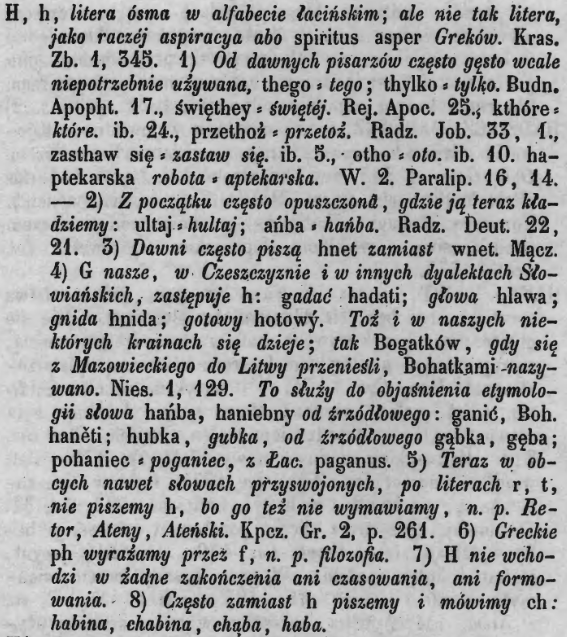
\includegraphics{H_Linde}
\bigskip

\url{http://teksty.klf.uw.edu.pl/26/3/LindeIIGP+2i.djvu?djvuopts=&page=169&zoom=width&showposition=0.2,0.28&highlight=2200,5000,131,193}

\bigskip
\newpage
\noindent H, h, \textit{litera ósma w alfabecie łacińskim}; \textit{ale nie tak litera}, \textit{jako raczéj aspiracya abo} \textlatin{spiritus asper} \textit{Greków}. \biblio{Kras. Zb.}{Ignacy Krasicki}{Zbior potrzebnieyszych wiadomości porządkiem alfabetu ułożonych.}{1, 345}. 
\begin{description}
\item[1)] \textit{Od dawnych pisarzów często gęsto wcale niepotrzebnie używana},
thego \doh{}  \textit{tego};
thylko \doh{} \textit{tylko}. \biblio{Budn. Apopht.}{Bieniasz Budny}{Krótkie a węzłowate powieści, które po grecku zową Apophtegmata}{17.},
święthey \doh{} \textit{świętéj}. \biblio{Rej. Apoc.}{Mikołaj Rej}{Apocalypsis}{25.},
kthóre \doh{} \textit{które}. \abbrv{\textlatin{ib.}}{ib. (ibidem) = tamże}{t} 24.,
przethoż \doh{} \textit{przetoż}. \biblio{Radz. Job.}{}{Biblia Brzeska, Księga Joba}{33, 1.},
zasthaw się \doh{} \textit{zastaw się}. \abbrv{\textlatin{ib.}}{ib. (ibidem) = tamże}{} 5.,
% Kropka występuje w skanie, nie ma jej w tekście OCR: · 
otho \doh{} \textit{oto}. \abbrv{\textlatin{ib.}}{ib. (ibidem) = tamże}{} 10.
haptekarska \textit{robota} \doh{} \textit{aptekarska}. \biblio{W. 2. Paralip.}{Jakub Wujek}{Biblia to iest księgi Starego y Nowego Testamentu, 2 Księga Kronik}{16, 14}. 

\item[--- 2)] \textit{Z początku często opuszczona}, \textit{gdzie ją teraz kładziemy}:
ultaj \doh{} \textit{hultaj};
ańba \doh{} \textit{hańba}. \biblio{Radz. Deut.}{}{Biblia Brzeska, Księga Powtórzonego Prawa}{22, 21}. 

\item[3)] \textit{Dawni często piszą} hnet \textit{zamiast} wnet. \biblio{Mącz.}{Jan Mączyński}{Lexicon Latino-Polonicum}{}
\item[4)] G \textit{nasze}, \textit{w Czeszczyznie i w innych dyalektach Słowiańskich}, \textit{zastępuje} h: 
\textit{gadać} \textczech{hadati}; 
\textit{glowa} \textczech{hlawa};
\textit{gnida} \textczech{hnida}; 
\textit{gotowy} \textczech{hotowý}. 
\textit{Toż i w naszych niektórych krainach się dzieje}; \textit{tak} Bogatków, \textit{gdy się z Mazowieckiego do Litwy przenieśli}, Bohatkami \textit{nazywano}. \biblio{Nies.}{Kasper Niesiecki}{Herbarz polski}{1, 129}.
\textit{To służy do objaśnienia etymologii słowa} hańba, haniebny \textit{od źrzódłowego}: ganić, \abbrv{Boh.}{Boh. = czeski}{t} \textczech{haněti}; 
hubka, \textit{gubka}, \textit{od źrzódłowego} gąbka, gęba;
pohaniec \doh{} \textit{poganiec}, \abbrv{\textit{z Łac}.}{z Łac. = z łaciny}{t} \textlatin{paganus}.

\item[5)] \textit{Teraz w obcych nawet słowach przyswojonych}, \textit{po literach} r, t,  \textit{nie piszemy} h, \textit{bo go też nie wymawiamy}, \abbrv{\textit{n}. \textit{p}.}{n. p. = na przykład}{t} \textit{Retor}, \textit{Ateny}, \textit{Ateński}. \biblio{Kpcz. Gr. 2}{Onufry Kopczyński SchP}{Gramatyka dla szkół narodowych na klassę 2}{\abbrv{\textlatin{p.}}{p. (pagina) = strona}{t} 261}.

\item[6)] \textit{Greckie} ph \textit{wyrażamy przez} f, \abbrv{\textit{n}. \textit{p}.}{n. p. = na przykład}{} \textit{filozofia}.

\item[7)] H \textit{nie wchodzi w żadne zakończenia ani czasowania}, \textit{ani formowania}.

\item[8)] \textit{Często zamiast} h \textit{piszemy i mówimy} ch\textit{:}
\textit{habina}, \textit{chabina}, \textit{chaba}, \textit{haba}.
\end{description}
\end{document}

%%% Local Variables: 
%%% coding: utf-8-unix
%%% TeX-engine: xetex 
%%% mode: latex
%%% TeX-master: t
%%% TeX-PDF-mode: t
%%% End: